
\section{syntax}

strong prefixing sull'input e sull'output


As we did whit multi $\pi$ calculus, we suppose that we have a countable set of names $\mathbb{N}$, ranged over by lower case letters $a,b, \cdots, z$. This names are used for communication channels and values. Furthermore we have a set of identifiers, ranged over by $A$. We represent the agents or processes by upper case letters $P,Q, \cdots $. A multi $\pi$ process, in addiction to the same actions of a $\pi$ process, can perform also a strong prefix:
\begin{center}
  $\pi$ ::= $\overline{x}y$ | $x(z)$ | $\underline{x(y)}$ | $\underline{\overline{x}y}$ | $\tau$ 
\end{center}
The process are defined, just as original $\pi$ calculus, by the following grammar:
\begin{center}
  \begin{tabular}{l}
    $P,Q$ ::= $0$ | $\pi.P$ | $P|Q$ | $P+Q$ | $(\nu x) P$ | $A(y_{1}, \cdots, y_{n})$
  \end{tabular}
\end{center}
and they have the same intuitive meaning as for the $\pi$ calculus. The strong prefix allows a process to make an atomic sequence of actions, so that more than one process can synchronize on this sequence. One can use the strong prefix only as an action prefixing for processes that can make at least a further action(perche'?).

Multi $\pi$ calculus is a conservative extension of the $\pi$ calculus in the sense that: any $\pi$ calculus process $p$ is also a multi $\pi$ calculus process and the semantic of $p$ according to the SOS rules of $\pi$ calculus is the same as the semantic of $p$ according to the SOS rules of multi $\pi$ calculus. 
We have to extend the following definition to deal with the strong prefix:
\begin{center}
  \begin{tabular}{ll}
	$bn(\underline{x(y)})\; =\; \{y\}$
      &
	$bn(\underline{\overline{x}y})\; =\; \emptyset$
    \\
	$fn(\underline{x(y)})\; =\; \{x\}$
      &
	$fn(\underline{\overline{x}y})\; =\; \{x,y\}$
    \\
  \end{tabular}
\end{center}


\section{early operational semantic with structural congruence}

The semantic of a multi $\pi$ process is labeled transition system such that
\begin{itemize}
  \item 
    the nodes are multi $\pi$ calculus process. The set of node is $\mathbb{P}_{m}$
  \item
    the actions are multi $\pi$ calculus actions. The set of actions is $\mathbb{A}_{m}$, we use $\alpha, \alpha_{1}, \alpha_{2},\cdots $ to range over the set of actions, we use $\sigma, \sigma_{1}, \sigma_{2}, \cdots $ to range over the set $\mathbb{A}_{m}^{+} \cup \{\tau\}$.
  \item
    the transition relations is $\rightarrow\subseteq \mathbb{P}_{m}\times (\mathbb{A}_{m}^{+} \cup \{\tau\})\times \mathbb{P}_{m}$
\end{itemize}

In this case, a label can be a sequence of prefixes, whether in the original $\pi$ calculus a label can be only a prefix. We use the symbol $\cdot$ to denote the concatenation operator.

\begin{definition}
  The \emph{early transition relation without structural congruence} is the smallest relation induced by the following rules:
  \begin{center}
    \begin{tabular}{ll}
 	  \bf{Out}
 	  \begin{tabular}{c}
 	      $\;\;$
 	    \\\hline
 	      $\overline{x}y.P \;\xrightarrow{\overline{x}y} P$
 	  \end{tabular}
	&
	  \bf{EInp}
	  \begin{tabular}{c}
	      $z\notin fn(P)$
	    \\\hline
	      $x(y).P \;\xrightarrow{xz} P\{z/y\}$
	  \end{tabular}
      \\\\
	  \bf{Tau}
	  \begin{tabular}{c}
	      $\;\;$
	    \\\hline
	      $\tau.P \;\xrightarrow{\tau} P$
	  \end{tabular}
	&
	  \bf{SInp}
	  \begin{tabular}{c}
	      $P \;\xrightarrow{\sigma} P^{'}\;\; \sigma\neq \tau$
	    \\\hline
	      $\underline{x(y)}.P \;\xrightarrow{xz \cdot \sigma} P^{'}\{z/y\}$
	  \end{tabular}
      \\\\
	  \bf{SOut}
	  \begin{tabular}{c}
	      $P \;\xrightarrow{\sigma} P^{'}\;\; \sigma\neq \tau$
	    \\\hline
	      $\underline{\overline{x}y}.P \;\xrightarrow{\overline{x}y \cdot \sigma} P^{'}$
	  \end{tabular}
	&
	$\inferrule* [left=\bf{Str}]{
	    P\equiv P^{'}
	  \\
	    P^{'}\; \;\xrightarrow{\alpha}\; Q^{'}
	  \\
	    Q\equiv Q^{'}
	}{
	    P\; \;\xrightarrow{\alpha}\; Q
	}$
      \\\\
	  \bf{Par}
	  \begin{tabular}{c}
	      $P \;\xrightarrow{\sigma} P^{'}\;\; bn(\sigma)\cap fn(Q)=\emptyset$
	    \\\hline
	      $P|Q \;\xrightarrow{\sigma} P^{'}|Q$
	  \end{tabular}
	&
	  $\inferrule* [left=\bf{Com}]{
	      P \;\xrightarrow{\sigma_{1}} P^{'}
	    \\
	      Q\;\xrightarrow{\sigma_{2}} Q^{'}
	    \\
	      Sync(\sigma_{1}, \sigma_{2}, \sigma_{3})
	  }{
	    P|Q \;\xrightarrow{\sigma_{3}} P^{'}|Q^{'}
	  }$
      \\\\
	  \bf{Res}
	  \begin{tabular}{c}
	      $P \;\xrightarrow{\sigma} P^{'}\;\; z\notin n(\alpha)$
	    \\\hline
	      $(\nu) z P \;\xrightarrow{\sigma} (\nu) z P^{'}$
	  \end{tabular}
	&
	  \bf{Sum}
	  \begin{tabular}{c}
	      $P \;\xrightarrow{\sigma} P^{'}$
	    \\\hline
	      $P+Q \;\xrightarrow{\sigma} P^{'}$
	  \end{tabular}
      \\\\
    \end{tabular}
  \end{center}
\end{definition}
\begin{definition}
  We define the synchronization relation in the following way:
  \begin{center}
    \begin{tabular}{ccc}
	  $\inferrule* [left=Com1L]{
	   }{
	    Sync(\overline{x}y,xy,\tau)
	  }$
	&
	  $\inferrule* [left=Com2L]{
	   }{
	    Sync(xy\cdot \sigma,\overline{x}y,\sigma)
	  }$	  
	&
      \\\\
	  $\inferrule* [left=Com1R]{
	   }{
	    Sync(xy,\overline{x}y,\tau)
	  }$
	&
	  $\inferrule* [left=Com2R]{
	   }{
	    Sync(\overline{x}y,xy\cdot \sigma,\sigma)
	  }$	  
	&
	  	
      \\\\
	  
	&
	  
	&
	  	
    \end{tabular}
  \end{center}
\end{definition}


\begin{example}
  We show an example of three processes that synchronize. In particular we prove that
  \begin{description}
    \item[Res]
      $(\nu x)((\underline{x(y)}.x(y).0|\overline{x}y.0)|\overline{x}y.0)\; 
	\;\xrightarrow{\tau}\; 
	  (\nu x)((0|0)|0)$
      \begin{description}
	\item
	  $x\notin n(\tau)$
	\item[Com]
	      $((\underline{x(y)}.x(y).0|\overline{x}y.0)|\overline{x}y.0)\; 
		\;\xrightarrow{\tau}\; 
		  ((0|0)|0)$
	      \begin{description}
	       \item[Com]
		  $\underline{x(y)}.x(y).0|\overline{x}y.0\; 
		    \;\xrightarrow{xy}\; 
		      0|0$
		  \begin{description}
		    \item[Com2L]
		      $Sync(xy\cdot xy,xy,xy)$
		    \item[Einp]
		      $\overline{x}y.0\; \;\xrightarrow{xy}\; 0$
		    \item[SOut]
		      $\underline{x(y)}.x(y).0\; 	
			\;\xrightarrow{xy\cdot xy}\; 
			  0$
		    \begin{description}
		      \item
			$x(y)\neq \tau$
		      \item[Out]
			$x(y).0\; 
			\;\xrightarrow{xy}\; 
			  0$
		    \end{description}
		  \end{description}
		\item[Out]
		  $\overline{x}y.0\; \;\xrightarrow{xy}\; 0$
		\item[Com1]
		  $Sync(xy,xy,\tau)$   
	      \end{description}
      \end{description}
  \end{description}
\end{example}


\begin{example}
  We want to prove that 
  \[
    (\underline{a(x)}.c(x).0|\overline{b}x.0)|(\overline{a}x.0|\underline{b(x)}.\overline{c}x.0)\;
      \;\xrightarrow{\tau}\; 
	(0|0)|(0|0)
  \]:
  \begin{description}
    \item[Str]
      $(\underline{a(x)}.c(x).0|\overline{b}x.0)|(\overline{a}x.0|\underline{b(x)}.\overline{c}x.0)\;
	\;\xrightarrow{\tau}\; 
	  (0|0)|(0|0)$
      \begin{description}
	\item[Com] 
	  $(\underline{a(x)}.c(x).0|\overline{a}x.0)|(\overline{b}x.0|\underline{b(x)}.\overline{c}x.0)\;
	    \;\xrightarrow{\tau}\;
	      (0|0)|(0|0)$
	  \begin{description}
	    \item[Com1R]
	      $Sync(cx, \overline{c}x, \tau)$
	    \item[Com]
	      $\overline{b}x.0|\underline{b(x)}.\overline{c}x.0\;
		\;\xrightarrow{\overline{c}x}\;
		  0|0$
	      \begin{description}
		\item[EInp]
		  $\overline{b}x.0
		    \;\xrightarrow{\overline{b}x}\;
		      0$
		\item[SOut]
		  $\underline{b(x)}.\overline{c}x.0\;
		    \;\xrightarrow{bx\cdot \overline{c}x}\;
		      0$
		  \begin{description}
		    \item[Out]
		      $\overline{c}x.0\;
			\;\xrightarrow{\overline{c}x}\;
			  0$
		  \end{description}
		\item[Com2R]
		  $Sync(\overline{b}x,bx\cdot \overline{c}x,\overline{c}x)$
	      \end{description}
	    \item[Com]
	      $\underline{a(x)}.c(x).0|\overline{a}x.0\;
		\;\xrightarrow{cx}\;
		  0|0$
	      \begin{description}
		\item[SOut]
		  $\underline{a(x)}.c(x).0\;
		    \;\xrightarrow{ax\cdot cx}\;
		      0$
		  \begin{description}
		    \item[Inp]
		      $c(x).0\;
			\;\xrightarrow{cx}\;
			  0$
		  \end{description}
		\item[Inp]
		  $\overline{a}x.0\;
		    \;\xrightarrow{ax}\;
		      0$
		\item[Com2L]
		  $Sync(ax\cdot cx, \overline{a}x, cx)$
	      \end{description}
	  \end{description}
	\item[]
	  $(\underline{a(x)}.c(x).0|\overline{b}x.0)|(\overline{a}x.0|\underline{b(x)}.\overline{c}x.0)\;
	    \equiv\;
	      (\underline{a(x)}.c(x).0|\overline{a}x.0)|(\overline{b}x.0|\underline{b(x)}.\overline{c}x.0)$
      \end{description}
  \end{description}
\end{example}


\begin{example}
  The \emph{dining philosophers} problem, originally proposed by Dijkstra in \cite{djkstra}, is defined in the following way: Five silent philosophers sit at a round table. There is one fork between each pair of adjacent philosophers. Each philosopher must alternately think and eat. However, a philosopher can only eat while holding both the fork to the left and the fork to the right. Each philosopher can pick up an adjacent fork, when available, and put it down, when holding it. The problem is to design an algorithm such that no philosopher will starve, i.e. can forever continue to alternate between eating and thinking. We present one solution which uses only two forks and two philosophers:
  \begin{itemize}
    \item
      we define two constants for the forks:
      \begin{center}
	\begin{tabular}{ll}
	    $fork_{1}\; \stackrel{def}{=}\; \overline{up_{1}}x.\overline{dn_{1}}x.fork_{1}$
	  &
	    $fork_{0}\; \stackrel{def}{=}\; \overline{up_{0}}x.\overline{dn_{0}}x.fork_{0}$
	\end{tabular}
      \end{center}
      the input name $x$ is not important and can be anything else.
    \item
      we define two constants for the philosophers:
      \begin{center}
	\begin{tabular}{l}
	    $phil_{1}\; \stackrel{def}{=}\; 
	      think(x).phil_{1}
	    +
	      \underline{up_{1}(x)}.up_{0}(x).eat(x).\underline{dn_{1}(x)}.dn_{0}(x).phil_{1}$
	  \\
	    $phil_{0}\; \stackrel{def}{=}\; 
	      think(x).phil_{0}
	    +
	      \underline{up_{0}(x)}.up_{1}(x).eat(x).\underline{dn_{0}(x)}.dn_{1}(x).phil_{0}$
	\end{tabular}
      \end{center}
      also in this case the name $x$ is not relevant.
    \item
      the following definition describe the whole system with philosophers and forks:
      \begin{center}
	$DP\; \stackrel{def}{=}\; (\nu \{up_{0}, up_{1}, down_{0}, down_{1}\})(phil_{0}|phil_{1}|fork_{0}|fork_{1})$
      \end{center}
      where with $(\nu \{up_{0}, up_{1}, down_{0}, down_{1}\})$ we mean $(\nu\; up_{0}) (\nu\; up_{1}) (\nu\; down_{0}) (\nu\; down_{1})$
    \item
      the operational semantic of $DP$ is the following lts:
      \begin{center}
	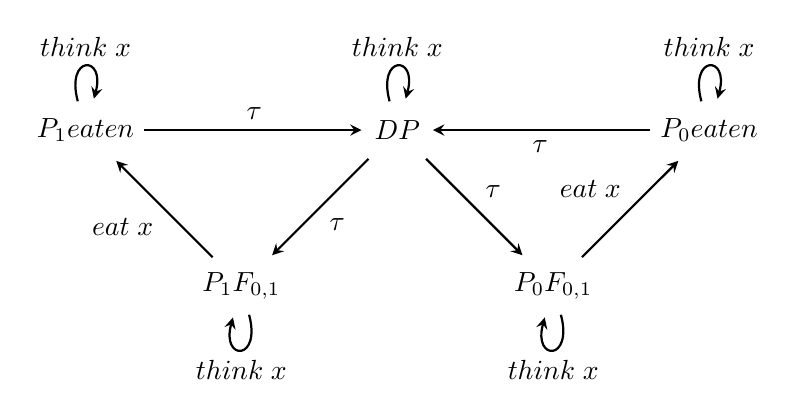
\begin{tikzpicture}[%
	    ->,
	    >=stealth,
	    shorten >=1pt,
	    node distance=2.8cm,
	    %on grid,
	    auto,
	    state/.append style={minimum size=2em},
	    thick
	  ]


  %\tikzstyle{every state}=[fill=red,draw=none,text=white]


	  \node[state] (A) {$P_{1}eaten$};
	  \node[state] (B) [below right of=A] {$P_{1}F_{0,1}$};
	  \node[state] (DP)[above right of=B] {$DP$};
	  \node[state] (C) [below right of=DP] {$P_{0}F_{0,1}$};
	  \node[state] (D) [above right of=C] {$P_{0}eaten$};
  
	  \path[->] 
	      
              (DP)       edge [loop above] node {$think\;x$} (DP)
			 edge              node {$\tau$} (C)
			 edge              node {$\tau$} (B)
	      (A)        edge [loop above] node {$think\;x$} (A)
			 edge              node {$\tau$} (DP)
	      (B)        edge [loop below] node {$think\;x$} (B)
			 edge   	   node {$eat\;x$} (A)
	      (C)        edge [loop below] node {$think\;x$} (C)
			 edge              node {$eat\;x$} (D)
	      (D)        edge [loop above] node {$think\;x$} (D)
			 edge              node {$\tau$} (DP);
         
      \end{tikzpicture}
    \end{center}
  \end{itemize}
  Now we need to prove every transition in the semantic of $DP$. Let $L=\{up_{0}, up_{1}, down_{0}, down_{1}\}$ we start with $DP\xrightarrow{\tau}DP$:



\end{example}

\begin{example}
  We want to show now an example of synchronization between four processes:
  \begin{description}
    \item[Res]
      $(\nu\; a)((((\underline{a(x)}.\underline{a(x)}.a(x).0| \overline{a}x.0)| \overline{a}x.0)| \overline{a}x.0)\;\;
	\xrightarrow{\tau}\;
	  (\nu\; a)(((0|0)|0)|0))$
      \begin{description}
	\item
	  $a\notin n(\tau)$
	\item[Com]
	  $((\underline{a(x)}.\underline{a(x)}.a(x).0| \overline{a}x.0)| \overline{a}x.0)| \overline{a}x.0\;\;
	    \xrightarrow{\tau}\;
	      ((0|0)|0)|0$
	  \begin{description}
	    \item[Com]
	      $(\underline{a(x)}.\underline{a(x)}.a(x).0| \overline{a}x.0)| \overline{a}x.0\;\;
		\xrightarrow{ax}\;
		   (0|0)|0$
	      \begin{description}
		\item[Com]
		  $\underline{a(x)}.\underline{a(x)}.a(x).0| \overline{a}x.0\;\;
		    \xrightarrow{ax\cdot ax}\;
		      0|0$
		  \begin{description}
		    \item[SOut]
		      $\underline{a(x)}.\underline{a(x)}.a(x).0\;\;
			  \xrightarrow{ax\cdot ax\cdot ax}\;
			    0$
		      \begin{description}
			\item[SOut]
			  $\underline{a(x)}.a(x).0\;\;
			    \xrightarrow{ax\cdot ax}\;
			      0$\newline
 			  %\begin{description}
 			  %   \item[SOut]
 				$\;\;\;\; {\bf SOut}\; \underline{a(x)}.a(x).0\;\;
				  \xrightarrow{ax\cdot ax}\;
				    0$\newline
	     			%\begin{description}
				%   \item[SOut]
				      .\hspace{4 mm}${\bf Out}\; a(x).0\;\;
					\xrightarrow{ax}\;
					   0$
				%\end{description}
 			  %\end{description}
		      \end{description}
		    \item[Inp]
		      $\overline{a}x.0\;\;\xrightarrow{\overline{a}x}\;0$
		    \item[Com2L]
		      $Sync(
			ax \cdot ax \cdot ax,
			\overline{a}x,
			ax \cdot ax
		      )$
		  \end{description}
		\item[Inp]
		  $\overline{a}x.0\;\;\xrightarrow{\overline{a}x}\;0$	 
		\item[Com2L]
		  $Sync(ax\cdot ax,\overline{a}x,ax)$
	      \end{description}
	    \item[Inp]
	      $\overline{a}x.0\;\;\xrightarrow{\overline{a}x}\;0$	      
	    \item[Com1L]
	      $Sync(ax,\overline{a}x,\tau)$
	  \end{description}
    \end{description}
  \end{description}

\end{example}



\section{late operational semantic with structural congruence}
% Definisci le regole late per Multi-pi. In questo caso credo sia indispensabile la restrizione sintattica che ti suggerivo(solo input nello strong prefixing e sincronizzazione solo con la prima), mentre mi pare che nel caso early dovrebbe funzionare anche il caso generale con Sync. 
\section{behavioural semantic}
\section{linear step sematics}
% Lo step successivo sarà di provare a definirsi una linear-step sematics per multi-pi, come fatto per multi-ccs. Non sono pero' molto persuaso che questo step sia facile da ottenere, e nemmeno se lo sia affatto.
\section{assiomatizzazione?}
\section{sistema di tipi?}